\documentclass[tikz,border=7pt]{standalone}
\usepackage{amsmath,pgfplots}
\pgfplotsset{compat=1.18}
\usetikzlibrary{arrows.meta,decorations.pathmorphing}
\definecolor{ink}{HTML}{21352F}\definecolor{teal}{HTML}{087F7B}
\definecolor{gold}{HTML}{C58B2A}\definecolor{blue}{HTML}{4B77A8}\definecolor{rose}{HTML}{B65A62}
\begin{document}
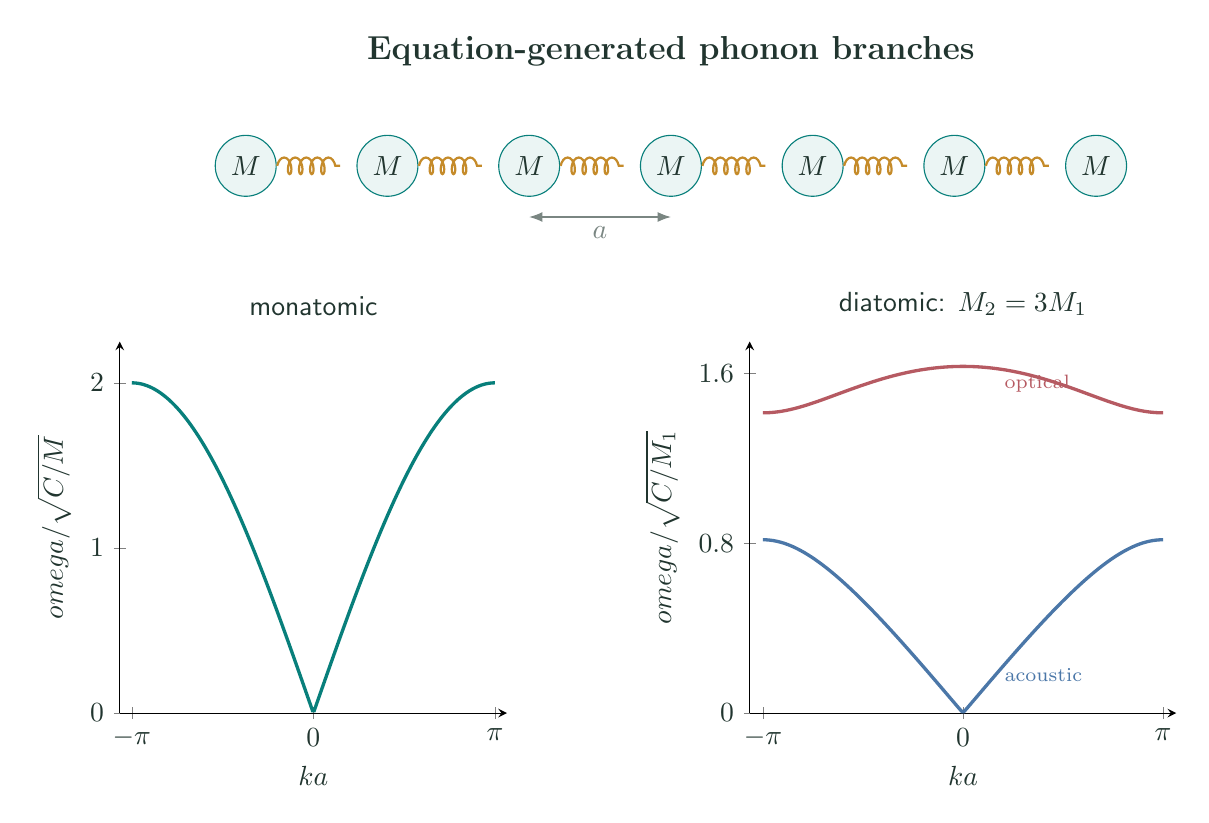
\begin{tikzpicture}[font=\sffamily,text=ink,>=Latex]
\node[font=\bfseries\large] at (0,5.1) {Equation-generated phonon branches};
\begin{scope}[yshift=3.65cm]
  \foreach \x in {-5.4,-3.6,-1.8,0,1.8,3.6,5.4}{\node[draw=teal,fill=teal!8,circle,minimum size=7mm] at (\x,0) {$M$};}
  \foreach \x in {-5.0,-3.2,-1.4,.4,2.2,4.0}{\draw[decorate,decoration={coil,segment length=4pt,amplitude=3pt},gold,thick] (\x,0)--++(.8,0);}
  \draw[<->,ink!60] (-1.8,-.65)--(0,-.65) node[midway,below] {$a$};
\end{scope}
\begin{axis}[at={(-7.0cm,-3.3cm)},anchor=south west,width=6.5cm,height=6.3cm,
 xmin=-3.35,xmax=3.35,ymin=0,ymax=2.25,axis lines=left,xlabel={$ka$},ylabel={$omega/\sqrt{C/M}$},
 xtick={-3.14159,0,3.14159},xticklabels={$-\pi$,$0$,$\pi$},ytick={0,1,2},title={monatomic}]
 \addplot[teal,very thick,domain=-3.14159:3.14159,samples=220]{2*abs(sin(deg(x)/2))};
\end{axis}
\begin{axis}[at={(1.0cm,-3.3cm)},anchor=south west,width=7.0cm,height=6.3cm,
 xmin=-3.35,xmax=3.35,ymin=0,ymax=1.75,axis lines=left,xlabel={$ka$},ylabel={$omega/\sqrt{C/M_1}$},
 xtick={-3.14159,0,3.14159},xticklabels={$-\pi$,$0$,$\pi$},ytick={0,.8,1.6},title={diatomic: $M_2=3M_1$}]
 \addplot[blue,very thick,domain=-3.14159:3.14159,samples=220]{sqrt(1.333333-sqrt(1.777777-1.333333*sin(deg(x)/2)^2))};
 \addplot[rose,very thick,domain=-3.14159:3.14159,samples=220]{sqrt(1.333333+sqrt(1.777777-1.333333*sin(deg(x)/2)^2))};
 \node[blue,font=\scriptsize,anchor=west] at (axis cs:.5,.18) {acoustic};
 \node[rose,font=\scriptsize,anchor=west] at (axis cs:.5,1.55) {optical};
\end{axis}
\end{tikzpicture}
\end{document}

